
%%--------------------------------------------------
%% Halliday: Fundamentals of Physics
%%--------------------------------------------------


%% Chapter 04: Motion in Two and Three Dimensions
%%--------------------------------------------------


%% Learning Objectives
%%--------------------------------------------------

%% 4.01: Draw two-dimensional and three-dimensional position vectors for a particle, indicating the components along the axes of a coordinate system.
%% 4.02: On a coordinate system, determine the direction and magnitude of a particle's position vector from its components, and vice versa.
%% 4.03: Apply the relationship between a particle's displacement vector and its initial and final position vectors.


%% Halliday Multiple Choice Questions
%%--------------------------------------------------
\element{halliday-mc}{
\begin{question}{halliday-ch04-q01}
    Velocity is defined as:
    \begin{choices}
      \correctchoice{rate of change of position with time}
        \wrongchoice{position divided by time}
        \wrongchoice{rate of change of acceleration with time}
        \wrongchoice{a speeding up or slowing down}
        \wrongchoice{change of position}
    \end{choices}
\end{question}
}

\element{halliday-mc}{
\begin{question}{halliday-ch04-q02}
    Acceleration is defined as:
    \begin{choices}
        \wrongchoice{rate of change of position with time}
        \wrongchoice{speed divided by time}
      \correctchoice{rate of change of velocity with time}
        \wrongchoice{a speeding up or slowing down}
        \wrongchoice{change of velocity}
    \end{choices}
\end{question}
}

\element{halliday-mc}{
\begin{question}{halliday-ch04-q03}
    Which of the following is a scalar quantity?
    \begin{choices}
      \correctchoice{Speed}
        \wrongchoice{Velocity}
        \wrongchoice{Displacement}
        \wrongchoice{Acceleration}
        \wrongchoice{None of the provided}
    \end{choices}
\end{question}
}

\element{halliday-mc}{
\begin{question}{halliday-ch04-q04}
    Which of the following is a vector quantity?
    \begin{choices}
        \wrongchoice{Mass}
        \wrongchoice{Density}
        \wrongchoice{Speed}
        \wrongchoice{Temperature}
      \correctchoice{None of the provided}
    \end{choices}
\end{question}
}

\element{halliday-mc}{
\begin{question}{halliday-ch04-q05}
    Which of the following is \emph{not} an example of accelerated motion?
    \begin{choices}
        \wrongchoice{Vertical component of projectile motion}
        \wrongchoice{Circular motion at constant speed}
        \wrongchoice{A swinging pendulum}
        \wrongchoice{Earth's motion about sun}
      \correctchoice{Horizontal component of projectile motion}
    \end{choices}
\end{question}
}

\element{halliday-mc}{
\begin{question}{halliday-ch04-q06}
    A particle goes from $x=\SI{-2}{\meter}$, $y=\SI{3}{\meter}$, $z=\SI{1}{\meter}$ to $x=\SI{3}{\meter}$, $y=\SI{-1}{\meter}$, $z=\SI{4}{\meter}$.
    Its displacement is:
    \begin{choices}
        \wrongchoice{$\left(\SI{1}{\meter}\right)\hat{\imath} + \left(\SI{2}{\meter}\right)\hat{\jmath} + \left(\SI{5}{\meter}\right)\hat{k}$}
      \correctchoice{$\left(\SI{5}{\meter}\right)\hat{\imath} − \left(\SI{4}{\meter}\right)\hat{\jmath} + \left(\SI{3}{\meter}\right)\hat{k}$}
        \wrongchoice{$-\left(\SI{5}{\meter}\right)\hat{\imath} + \left(\SI{4}{\meter}\right)\hat{\jmath} − \left(\SI{3}{\meter}\right)\hat{k}$}
        \wrongchoice{$-\left(\SI{1}{\meter}\right)\hat{\imath} − \left(\SI{2}{\meter}\right)\hat{\jmath} − \left(\SI{5}{\meter}\right)\hat{k}$}
        \wrongchoice{$-\left(\SI{5}{\meter}\right)\hat{\imath} − \left(\SI{2}{\meter}\right)\hat{\jmath} + \left(\SI{3}{\meter}\right)\hat{k}$}
    \end{choices}
\end{question}
}

\element{halliday-mc}{
\begin{question}{halliday-ch04-q07}
    A jet plane in straight horizontal flight passes over your head. 
    When it is directly above you,
        the sound seems to come from a point behind the plane in a direction \ang{30} from the vertical.
    The speed of the plane is:
    \begin{choices}
        \wrongchoice{the same as the speed of sound}
      \correctchoice{half the speed of sound}
        \wrongchoice{three-fifths the speed of sound}
        \wrongchoice{0.866 times the speed of sound}
        \wrongchoice{twice the speed of sound}
    \end{choices}
\end{question}
}

\element{halliday-mc}{
\begin{question}{halliday-ch04-q08}
    A plane traveling north at \SI{200}{\meter\per\second} turns and then travels south at \SI{200}{\meter\per\second}.
    The change in its velocity is:
    \begin{multicols}{2}
    \begin{choices}
        \wrongchoice{zero}
        \wrongchoice{\SI{200}{\meter\per\second} north}
        \wrongchoice{\SI{200}{\meter\per\second} south}
        \wrongchoice{\SI{400}{\meter\per\second} north}
      \correctchoice{\SI{400}{\meter\per\second} south}
    \end{choices}
    \end{multicols}
\end{question}
}

\element{halliday-mc}{
\begin{question}{halliday-ch04-q09}
    Two bodies are falling with negligible air resistance, side by side, above a horizontal plane. 
    If one of the bodies is given an additional horizontal acceleration during its descent, it:
    \begin{choices}
      \correctchoice{strikes the plane at the same time as the other body}
        \wrongchoice{strikes the plane earlier than the other body}
        \wrongchoice{has the vertical component of its velocity altered}
        \wrongchoice{has the vertical component of its acceleration altered}
        \wrongchoice{follows a straight line path along the resultant acceleration vector}
    \end{choices}
\end{question}
}

\element{halliday-mc}{
\begin{question}{halliday-ch04-q10}
    The velocity of a projectile equals its initial velocity added to:
    \begin{choices}
        \wrongchoice{a constant horizontal velocity}
        \wrongchoice{a constant vertical velocity}
        \wrongchoice{a constantly increasing horizontal velocity}
      \correctchoice{a constantly increasing downward velocity}
        \wrongchoice{a constant velocity directed at the target}
    \end{choices}
\end{question}
}

\element{halliday-mc}{
\begin{question}{halliday-ch04-q11}
    A stone thrown from the top of a tall building follows a path that is:
    \begin{choices}
        \wrongchoice{circular}
        \wrongchoice{made of two straight line segments}
        \wrongchoice{hyperbolic}
      \correctchoice{parabolic}
        \wrongchoice{a straight line}
    \end{choices}
\end{question}
}

\element{halliday-mc}{
\begin{questionmult}{halliday-ch04-q12}
    Identical guns fire identical bullets horizontally at the same speed from the same height above level planes,
        one on the Earth and one on the Moon.
    Which of the following three statements is/are true?
    \begin{choices}
      \correctchoice{The horizontal distance traveled by the bullet is greater for the Moon.}
      \correctchoice{The flight time is less for the bullet on the Earth.}
        \wrongchoice{The velocity of the bullets at impact are the same.}
        %% A. III only
        %% B. I and II only
        %% C. I and III only
        %% D. II and III only
        %% E. I, II, III
        %% ans: B
    \end{choices}
\end{questionmult}
}

\element{halliday-mc}{
\begin{question}{halliday-ch04-q13}
    A stone is thrown horizontally and follows the path $XYZ$ shown. 
    \begin{center}
    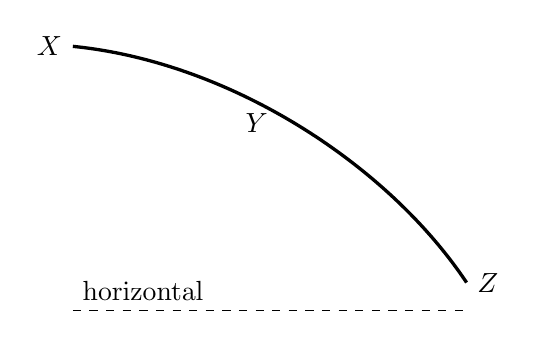
\begin{tikzpicture}
        %% Path
        \draw[very thick] (0,3) .. controls (2,2.8) and (4,1.5) .. (5,0)
            node[pos=0.0,anchor=east] {$X$}
            node[pos=0.4,anchor=north] {$Y$}
            node[pos=1.0,anchor=west] {$Z$};
        %% Horizontal
        \draw[dashed] (0,-1em) -- (5,-1em) node[pos=0.0,anchor=south west] {horizontal};
    \end{tikzpicture}
    \end{center}
    The direction of the acceleration of the stone at point $Y$ is:
    \begin{multicols}{3}
    \begin{choices}
        \AMCboxDimensions{down=-0.3cm}
        %% ANS is A
        \correctchoice{
            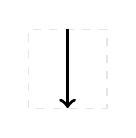
\begin{tikzpicture}
                \draw[draw=white!90!black,dashed] (-0.5,0.0) rectangle (+0.5,1.0);
                \draw[very thick,->] (0,1) -- ++(270:1);
            \end{tikzpicture}
        }
        \wrongchoice{
            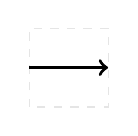
\begin{tikzpicture}
                \draw[draw=white!90!black,dashed] (0.0,0.0) rectangle (1,1);
                \draw[very thick,->] (0,0.5) -- ++(0:1);
            \end{tikzpicture}
        }
        \wrongchoice{
            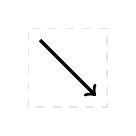
\begin{tikzpicture}
                \draw[draw=white!90!black,dashed] (0.0,0.0) rectangle (1,1);
                \draw[very thick,->] (0.15,0.85) -- ++(-45:1);
            \end{tikzpicture}
        }
        \wrongchoice{
            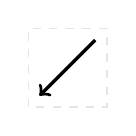
\begin{tikzpicture}
                \draw[draw=white!90!black,dashed] (0.0,0.0) rectangle (1,1);
                \draw[very thick,->] (0.85,0.85) -- ++(225:1);
            \end{tikzpicture}
        }
        \wrongchoice{
            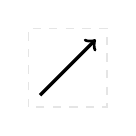
\begin{tikzpicture}
                \draw[draw=white!90!black,dashed] (0.0,0.0) rectangle (1,1);
                \draw[very thick,->] (0.15,0.15) -- ++(+45:1);
            \end{tikzpicture}
        }
        %% Added for Symmetry
        \wrongchoice{
            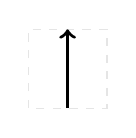
\begin{tikzpicture}
                \draw[draw=white!90!black,dashed] (-0.5,0.0) rectangle (+0.5,1.0);
                \draw[very thick,->] (0,0) -- ++(90:1);
            \end{tikzpicture}
        }
    \end{choices}
    \end{multicols}
\end{question}
}

\element{halliday-mc}{
\begin{question}{halliday-ch04-q14}
    A bullet shot horizontally from a gun:
    \begin{choices}
        \wrongchoice{strikes the ground much later than one dropped vertically from the same point at the same instant}
        \wrongchoice{never strikes the ground}
      \correctchoice{strikes the ground at approximately the same time as one dropped vertically from the same point at the same instant}
        \wrongchoice{travels in a straight line}
        \wrongchoice{strikes the ground much sooner than one dropped from the same point at the same instant}
    \end{choices}
\end{question}
}

\element{halliday-mc}{
\begin{question}{halliday-ch04-q15}
    A bomber flying in level flight with constant velocity releases a bomb before it is over the target.
    Neglecting air resistance,
        which one of the following is \emph{not} true?
    \begin{choices}
        \wrongchoice{The bomber is over the target when the bomb strikes}
        \wrongchoice{The acceleration of the bomb is constant}
      \correctchoice{The horizontal velocity of the plane equals the vertical velocity of the bomb when it hits the target}
        \wrongchoice{The bomb travels in a curved path}
        \wrongchoice{The time of flight of the bomb is independent of the horizontal speed of the plane}
    \end{choices}
\end{question}
}

\element{halliday-mc}{
\begin{question}{halliday-ch04-q16}
    The airplane shown is in level flight at an altitude of \SI{0.50}{\kilo\meter} and a speed of \SI{150}{\kilo\meter\per\hour}.
    \begin{center}
    \begin{tikzpicture}
        \node[anchor=north,fill,pattern=north east lines,minimum width=6.4cm, minimum height=0.05cm] at (0,0) {};
        \draw (-3.2,0) -- (3.2,0);
        \draw[fill] (3.0,0) circle (1.5pt) node[anchor=south] {$X$};
        %% Distance
        \draw[<->] (-3,0) -- (-3,2) node[pos=0.5,anchor=center,fill=white] {\SI{0.5}{\kilo\meter}};
        \draw[<->] (+3,-0.75) -- (-1,-0.75) node[pos=0.5,anchor=center,fill=white] {$d$};
        %% Airplace
        \node[draw,fill=white!90!black,rectangle,anchor=south,minimum size=0.5cm] (A) at (-3,2) {};
        \draw[thick,->] (A.east) -- ++(0:2cm) node[anchor=south,pos=0.5] {\SI{150}{\kilo\meter\per\hour}};
    \end{tikzpicture}
    \end{center}
    At what distance $d$ should it release a heavy bomb to hit the target $X$? 
    Take $g=\SI{10}{\meter\per\second\squared}$.
    \begin{multicols}{3}
    \begin{choices}
        \wrongchoice{\SI{150}{\meter}}
        \wrongchoice{\SI{295}{\meter}}
      \correctchoice{\SI{420}{\meter}}
        \wrongchoice{\SI{2550}{\meter}}
        \wrongchoice{\SI{15 000}{\meter}}
    \end{choices}
    \end{multicols}
\end{question}
}

\element{halliday-mc}{
\begin{question}{halliday-ch04-q17}
    An object is shot from the back of a railroad flatcar moving at \SI{40}{\kilo\meter\per\hour} on a straight horizontal road.
    The launcher is aimed upward, perpendicular to the bed of the flatcar.
    The object falls:
    \begin{choices}
        \wrongchoice{in front of the flatcar}
        \wrongchoice{behind the flatcar}
      \correctchoice{on the flatcar}
        \wrongchoice{either behind or in front of the flatcar, depending on the initial speed of the object}
        \wrongchoice{to the side of the flatcar}
    \end{choices}
\end{question}
}

\element{halliday-mc}{
\begin{question}{halliday-ch04-q18}
    A ball is thrown horizontally from the top of a \SI{20}{\meter} high hill. 
    \begin{center}
    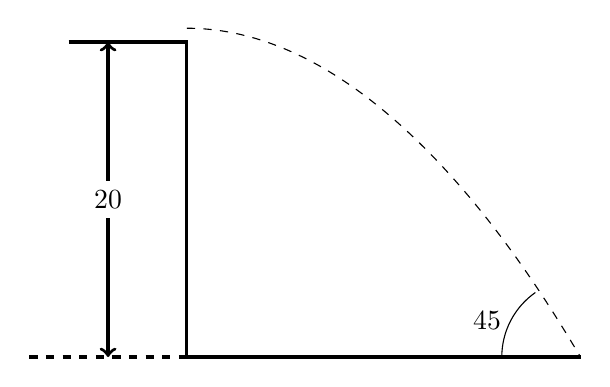
\begin{tikzpicture}
        %% Surface
        \draw[very thick] (-1.5,0) -- (0,0) -- (0,-4) -- (5,-4);
        \draw[very thick,dashed] (-2,-4) -- (0,-4);
        \node (A) at (-1,-2.0) {\SI{20}{\meter}};
        \draw[very thick,->] (A) -- (-1,0);
        \draw[very thick,->] (A) -- (-1,-4);
        %% Trajectory
        \draw[dashed] (0,5pt) parabola bend (0,5pt) (5,-4);
        \draw (5,-4) ++ (180:1) arc(180:125:1) node[pos=0.5,anchor=east] {\ang{45}};
    \end{tikzpicture}
    \end{center}
    It strikes the ground at an angle of \ang{45}.
        With what speed was it thrown?
    \begin{multicols}{3}
    \begin{choices}
        \wrongchoice{\SI{14}{\meter\per\second}}
      \correctchoice{\SI{20}{\meter\per\second}}
        \wrongchoice{\SI{28}{\meter\per\second}}
        \wrongchoice{\SI{32}{\meter\per\second}}
        \wrongchoice{\SI{40}{\meter\per\second}}
    \end{choices}
    \end{multicols}
\end{question}
}

\element{halliday-mc}{
\begin{question}{halliday-ch04-q19}
    A stone is thrown outward from the top of a \SI{59.4}{\meter} high cliff with an upward velocity component of \SI{19.5}{\meter\per\second}. 
    How long is stone in the air?
    \begin{multicols}{3}
    \begin{choices}
        \wrongchoice{\SI{4.00}{\second}}
        \wrongchoice{\SI{5.00}{\second}}
      \correctchoice{\SI{6.00}{\second}}
        \wrongchoice{\SI{7.00}{\second}}
        \wrongchoice{\SI{8.00}{\second}}
    \end{choices}
    \end{multicols}
\end{question}
}

\element{halliday-mc}{
\begin{question}{halliday-ch04-q20}
    A large cannon is fired from ground level over level ground at an angle of \ang{30} above the horizontal.
    The muzzle speed is \SI{980}{\meter\per\second}.
    Neglecting air resistance,
        the projectile will travel what horizontal distance before striking the ground?
    \begin{multicols}{3}
    \begin{choices}
        \wrongchoice{\SI{4.3}{\kilo\meter}}
        \wrongchoice{\SI{8.5}{\kilo\meter}}
        \wrongchoice{\SI{43}{\kilo\meter}}
      \correctchoice{\SI{85}{\kilo\meter}}
        \wrongchoice{\SI{170}{\kilo\meter}}
    \end{choices}
    \end{multicols}
\end{question}
}

\element{halliday-mc}{
\begin{question}{halliday-ch04-q21}
    A boy on the edge of a vertical cliff \SI{20}{\meter} high throws a stone horizontally outward with a speed of \SI{20}{\meter\per\second}. 
    It strikes the ground at what horizontal distance from the foot of the cliff?
    Use $g=\SI{10}{\meter\per\second\squared}$.
    \begin{multicols}{2}
    \begin{choices}
        \wrongchoice{\SI{10}{\meter}}
      \correctchoice{\SI{40}{\meter}}
        \wrongchoice{\SI{50}{\meter}}
        \wrongchoice{\SI[parse-numbers=false]{50\sqrt{5}}{\meter}}
        \wrongchoice{none of the provided}
    \end{choices}
    \end{multicols}
\end{question}
}

\element{halliday-mc}{
\begin{question}{halliday-ch04-q22}
    Which of the curves on the graph below best represents the vertical component $v_y$ of the velocity versus the time $t$ for a projectile fired at an angle of \ang{45} above the horizontal?
    \begin{center}
    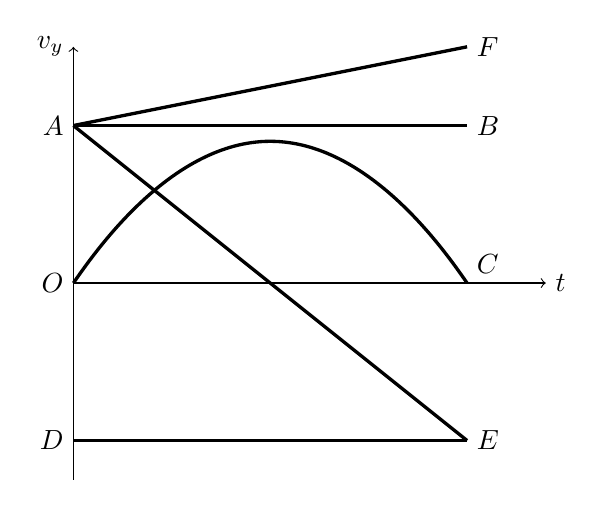
\begin{tikzpicture}
        %% Axis
        \draw[->] (0,-2.5) -- (0,3) node[anchor=east] {$v_y$};
        \draw[->] (0,0) -- (6,0) node[anchor=west] {$t$};
        %% Left Labels
        \node[anchor=east] at (0,+2) {$A$};
        \node[anchor=east] at (0,+0) {$O$};
        \node[anchor=east] at (0,-2) {$D$};
        %% Right Labels
        \node[anchor=west] at (5,+3) {$F$};
        \node[anchor=west] at (5,+2) {$B$};
        \node[anchor=south west] at (5,0) {$C$};
        \node[anchor=west] at (5,-2) {$E$};
        %% Paths
        \draw[very thick] (0,-2) -- (5,-2); %%DE
        \draw[very thick] (0,+2) -- (5,-2); %%AE
        \draw[very thick] (0,0)  parabola bend (2.5,1.8) (5,0); %%OC
        \draw[very thick] (0,+2) -- (5,+2); %%AB
        \draw[very thick] (0,+2) -- (5,+3); %%AF
    \end{tikzpicture}
    \end{center}
    \begin{multicols}{3}
    \begin{choices}
        \wrongchoice{OC}
        \wrongchoice{DE}
        \wrongchoice{AB}
      \correctchoice{AE}
        \wrongchoice{AF}
    \end{choices}
    \end{multicols}
\end{question}
}

%\element{halliday-mc}{
%\begin{question}{halliday-ch04-q23}
%    A cannon fires a projectile as shown. 
%    The dashed line shows the trajectory in the absence of gravity;
%        points $MNOP$ correspond to the position of the projectile at one second intervals. 
%    \begin{center}
%    \begin{tikzpicture}
%        %% NOTE; graph
%    \end{tikzpicture}
%    \end{center}
%    If $g=\SI{10}{\meter\per\second\squared}$,
%        the lengths $X$, $Y$, $Z$ are:
%    \begin{multicols}{2}
%    \begin{choices}
%        \wrongchoice{\SI{5}{\meter},    \SI{10}{\meter},    \SI{15}{\meter}}
%      \correctchoice{\SI{5}{\meter},    \SI{20}{\meter},    \SI{45}{\meter}}
%        \wrongchoice{\SI{10}{\meter},   \SI{40}{\meter},    \SI{90}{\meter}}
%        \wrongchoice{\SI{10}{\meter},   \SI{20}{\meter},    \SI{30}{\meter}}
%        \wrongchoice{\SI{0.2}{\meter},  \SI{0.8}{\meter},   \SI{1.8}{\meter}}
%    \end{choices}
%    \end{multicols}
%\end{question}
%}

%\element{halliday-mc}{
%\begin{question}{halliday-ch04-q24}
%    A dart is thrown horizontally toward $X$ at \SI{20}{\meter\per\second} as shown. 
%    \begin{center}
%    \begin{tikzpicture}
%        %% NOTE; graph
%    \end{tikzpicture}
%    \end{center}
%    It hits $Y$ \SI{0.1}{\second} later. 
%    The distance $XY$ is:
%    \begin{multicols}{3}
%    \begin{choices}
%        \wrongchoice{\SI{2}{\meter}}
%        \wrongchoice{\SI{1}{\meter}}
%        \wrongchoice{\SI{0.5}{\meter}}
%        \wrongchoice{\SI{0.1}{\meter}}
%      \correctchoice{\SI{0.05}{\meter}}
%    \end{choices}
%    \end{multicols}
%\end{question}
%}

\element{halliday-mc}{
\begin{question}{halliday-ch04-q25}
    A projectile is fired from ground level over level ground with an initial velocity that has a vertical component of \SI{20}{\meter\per\second} and a horizontal component of \SI{30}{\meter\per\second}.
    Using $g=\SI{10}{\meter\per\second\squared}$,
        the distance from launching to landing points is:
    \begin{multicols}{3}
    \begin{choices}
        \wrongchoice{\SI{40}{\meter}}
        \wrongchoice{\SI{60}{\meter}}
        \wrongchoice{\SI{80}{\meter}}
      \correctchoice{\SI{120}{\meter}}
        \wrongchoice{\SI{180}{\meter}}
    \end{choices}
    \end{multicols}
\end{question}
}

\element{halliday-mc}{
\begin{question}{halliday-ch04-q26}
    An object, tied to a string,
        moves in a circle at constant speed on a horizontal surface as shown.
    \begin{center}
    \begin{tikzpicture}
        %% Circle
        \draw[dashed] (0,0) circle (2cm);
        %% Points
        \draw[fill] (0:2) circle (1.5pt) node[anchor=west] {$Z$};
        \draw[fill] (90:2) circle (1.5pt) node[anchor=south] {$W$};
        \draw[fill] (180:2) circle (1.5pt) node[anchor=east] {$X$};
        \draw[fill] (270:2) circle (1.5pt) node[anchor=north] {$Y$};
        %% Object
        \draw (0,0) -- (315:2);
        \draw[fill] (315:2) circle (0.5ex); 
        \draw[thick,->] (290:2.3) arc (290:340:2.3);
    \end{tikzpicture}
    \end{center}
    The direction of the displacement of this object,
        as it travels from $W$ to $X$ is:
    \begin{multicols}{3}
    \begin{choices}
        \wrongchoice{
            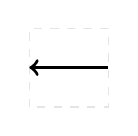
\begin{tikzpicture}
                \draw[draw=white!90!black,dashed] (-0.5,0.0) rectangle (+0.5,1.0);
                \draw[very thick,->] (0.5,0.5) -- ++(180:1);
            \end{tikzpicture}
        }
        \wrongchoice{
            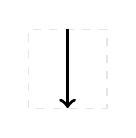
\begin{tikzpicture}
                \draw[draw=white!90!black,dashed] (-0.5,0.0) rectangle (+0.5,1.0);
                \draw[very thick,->] (0,1) -- ++(270:1);
            \end{tikzpicture}
        }
        \wrongchoice{
            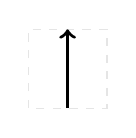
\begin{tikzpicture}
                \draw[draw=white!90!black,dashed] (-0.5,0.0) rectangle (+0.5,1.0);
                \draw[very thick,->] (0,0) -- ++(90:1);
            \end{tikzpicture}
        }
        \wrongchoice{
            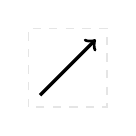
\begin{tikzpicture}
                \draw[draw=white!90!black,dashed] (0.0,0.0) rectangle (1,1);
                \draw[very thick,->] (0.15,0.15) -- ++(+45:1);
            \end{tikzpicture}
        }
        %% ANS is E
        \correctchoice{
            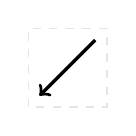
\begin{tikzpicture}
                \draw[draw=white!90!black,dashed] (0.0,0.0) rectangle (1,1);
                \draw[very thick,->] (0.85,0.85) -- ++(225:1);
            \end{tikzpicture}
        }
        %% Added for Symmetry
        \wrongchoice{
            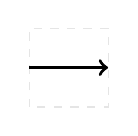
\begin{tikzpicture}
                \draw[draw=white!90!black,dashed] (0.0,0.0) rectangle (1,1);
                \draw[very thick,->] (0,0.5) -- ++(0:1);
            \end{tikzpicture}
        }
    \end{choices}
    \end{multicols}
\end{question}
}

\element{halliday-mc}{
\begin{question}{halliday-ch04-q27}
    A toy racing car moves with constant speed around the circle shown below. 
    \begin{center}
    \begin{tikzpicture}
        %% Axis
        \draw[dashed] (-3,0) -- (3,0) node[pos=1.0,anchor=north] {$x$};
        \draw[dashed] (0,-3) -- (0,3) node[pos=1.0,anchor=east] {$y$};
        %% Cirlce
        \draw (0,0) circle (2cm);
        %% Points
        \draw[fill] (90:2) circle (1.5pt) node[anchor=south west] {$A$};
        \draw[fill] (180:2) circle (1.5pt) node[anchor=south east] {$B$};
    \end{tikzpicture}
    \end{center}
    When it is at point $A$ its coordinates are $x=0$, $y=\SI{3}{\meter}$ and its velocity is $\left(\SI{6}{\meter\per\second}\right)\hat{\imath}$. 
    When it is at point $B$ its velocity and acceleration are:
    \begin{choices}
        \wrongchoice{$-\left(\SI{6}{\meter\per\second}\right)\hat{\jmath}$ and $\left(\SI{12}{\meter\per\second}\right)\hat{\imath}$, respectively}
        \wrongchoice{$\left(\SI{6}{\meter\per\second}\right)\hat{\imath}$ and  $-\left(\SI{2}{\meter\per\second}\right)\hat{\imath}$, respectively}
      \correctchoice{$\left(\SI{6}{\meter\per\second}\right)\hat{\jmath}$ and  $\left(\SI{12}{\meter\per\second}\right)\hat{\imath}$, respectively}
        \wrongchoice{$\left(\SI{6}{\meter\per\second}\right)\hat{\imath}$ and  $\left(\SI{2}{\meter\per\second}\right)\hat{\jmath}$, respectively}
        \wrongchoice{$\left(\SI{6}{\meter\per\second}\right)\hat{\jmath}$ and  $0$, respectively}
    \end{choices}
\end{question}
}

\element{halliday-mc}{
\begin{question}{halliday-ch04-q28}
    An airplane makes a gradual \ang{90} turn while flying at a constant speed of \SI{200}{\meter\per\second}. 
    The process takes \SI{20.0}{\second} to complete. 
    For this turn the magnitude of the average acceleration of the plane is:
    \begin{multicols}{3}
    \begin{choices}
        \wrongchoice{zero}
        \wrongchoice{\SI{40}{\meter\per\second\squared}}
        \wrongchoice{\SI{20}{\meter\per\second\squared}}
      \correctchoice{\SI{14}{\meter\per\second\squared}}
        \wrongchoice{\SI{10}{\meter\per\second\squared}}
    \end{choices}
    \end{multicols}
\end{question}
}

\element{halliday-mc}{
\begin{question}{halliday-ch04-q29}
    An airplane is flying north at \SI{500}{\kilo\meter\per\hour}. 
    It makes a gradual \ang{180} turn at constant speed,
        changing its direction of travel from north through east to south. 
    The process takes \SI{40}{\second}. 
    The average acceleration of the plane for this turn is:
    \begin{multicols}{2}
    \begin{choices}
        \wrongchoice{\SI{12.5}{\kilo\meter\per\hour\per\second}, north}
        \wrongchoice{\SI{12.5}{\kilo\meter\per\hour\per\second}, east}
        \wrongchoice{\SI{12.5}{\kilo\meter\per\hour\per\second}, south}
        \wrongchoice{\SI{25}{\kilo\meter\per\hour\per\second}, north}
      \correctchoice{\SI{25}{\kilo\meter\per\hour\per\second}, south}
    \end{choices}
    \end{multicols}
\end{question}
}

\element{halliday-mc}{
\begin{question}{halliday-ch04-q30}
    An object is moving on a circular path of radius $\pi$ meters at a constant speed of \SI{4.0}{\meter\per\second}. 
    The time required for one revolution is:
    \begin{multicols}{3}
    \begin{choices}
        \wrongchoice{$\dfrac{2}{\pi^2}\,\si{\second}$}
      \correctchoice{$\dfrac{\pi^2}{2}\,\si{\second}$}
        \wrongchoice{$\dfrac{\pi}{2}\,\si{\second}$}
        \wrongchoice{$\dfrac{\pi^2}{4}\,\si{\second}$}
        \wrongchoice{$\dfrac{2}{\pi}\,\si{\second}$}
    \end{choices}
    \end{multicols}
\end{question}
}

\element{halliday-mc}{
\begin{question}{halliday-ch04-q31}
    A particle moves at constant speed in a circular path. 
    The instantaneous velocity and instantaneous acceleration vectors are:
    \begin{choices}
        \wrongchoice{both tangent to the circular path}
        \wrongchoice{both perpendicular to the circular path}
      \correctchoice{perpendicular to each other}
        \wrongchoice{opposite to each other}
        \wrongchoice{none of the provided}
    \end{choices}
\end{question}
}

\element{halliday-mc}{
\begin{question}{halliday-ch04-q32}
    A stone is tied to a string and whirled at constant speed in a horizontal circle. 
    The speed is then doubled without changing the length of the string. 
    Afterward the magnitude of the acceleration of the stone is:
    \begin{multicols}{2}
    \begin{choices}
        \wrongchoice{the same}
        \wrongchoice{twice as great}
      \correctchoice{four times as great}
        \wrongchoice{half as great}
        \wrongchoice{one-fourth as great}
    \end{choices}
    \end{multicols}
\end{question}
}

\element{halliday-mc}{
\begin{question}{halliday-ch04-q33}
    Two objects are traveling around different circular orbits with constant speed. 
    They both have the same acceleration but object $A$ is traveling twice as fast as object $B$. 
    The orbit radius for object $A$ is \rule[-0.1pt]{4em}{0.1pt} the orbit radius for object $B$.
    \begin{multicols}{2}
    \begin{choices}
        \wrongchoice{one-fourth}
        \wrongchoice{one-half}
        \wrongchoice{the same as}
        \wrongchoice{twice}
      \correctchoice{four times}
    \end{choices}
    \end{multicols}
\end{question}
}

\element{halliday-mc}{
\begin{question}{halliday-ch04-q34}
    A stone is tied to a 0.50-m string and whirled at a constant speed of \SI{4.0}{\meter\per\second} in a vertical circle.
    Its acceleration at the top of the circle is:
    \begin{multicols}{2}
    \begin{choices}
        \wrongchoice{\SI{9.8}{\meter\per\second\squared}, up}
        \wrongchoice{\SI{9.8}{\meter\per\second\squared}, down}
        \wrongchoice{\SI{8.0}{\meter\per\second\squared}, down}
        \wrongchoice{\SI{32}{\meter\per\second\squared}, up}
      \correctchoice{\SI{32}{\meter\per\second\squared}, down}
    \end{choices}
    \end{multicols}
\end{question}
}

\element{halliday-mc}{
\begin{question}{halliday-ch04-q35}
    A stone is tied to a \SI{0.50}{\meter} string and whirled at a constant speed of \SI{4.0}{\meter\per\second} in a vertical circle.
    Its acceleration at the bottom of the circle is:
    \begin{multicols}{2}
    \begin{choices}
        \wrongchoice{\SI{9.8}{\meter\per\second\squared}, up}
        \wrongchoice{\SI{9.8}{\meter\per\second\squared}, down}
        \wrongchoice{\SI{8.0}{\meter\per\second\squared}, up}
      \correctchoice{\SI{32}{\meter\per\second\squared}, up}
        \wrongchoice{\SI{32}{\meter\per\second\squared}, down}
    \end{choices}
    \end{multicols}
\end{question}
}

\element{halliday-mc}{
\begin{question}{halliday-ch04-q36}
    A car rounds a \SI{20}{\meter} radius curve at \SI{10}{\meter\per\second}. 
    The magnitude of its acceleration is:
    \begin{multicols}{2}
    \begin{choices}
        \wrongchoice{zero}
        \wrongchoice{\SI{0.20}{\meter\per\second\squared}}
      \correctchoice{\SI{5.0}{\meter\per\second\squared}}
        \wrongchoice{\SI{40}{\meter\per\second\squared}}
        \wrongchoice{\SI{400}{\meter\per\second\squared}}
    \end{choices}
    \end{multicols}
\end{question}
}

\element{halliday-mc}{
\begin{question}{halliday-ch04-q37}
    For a biological sample in a \SI{1.0}{\meter} radius centrifuge to have a centripetal acceleration of $25g$ its speed must be:
    \begin{multicols}{3}
    \begin{choices}
        \wrongchoice{\SI{11}{\meter\per\second}}
      \correctchoice{\SI{16}{\meter\per\second}}
        \wrongchoice{\SI{50}{\meter\per\second}}
        \wrongchoice{\SI{122}{\meter\per\second}}
        \wrongchoice{\SI{245}{\meter\per\second}}
    \end{choices}
    \end{multicols}
\end{question}
}

\element{halliday-mc}{
\begin{question}{halliday-ch04-q38}
    A girl jogs around a horizontal circle with a constant speed. 
    She travels one fourth of a revolution,
        a distance of \SI{25}{\meter} along the circumference of the circle,
        in \SI{5.0}{\second}.
    The magnitude of her acceleration is:
    \begin{multicols}{3}
    \begin{choices}
        \wrongchoice{\SI{0.31}{\meter\per\second\squared}}
        \wrongchoice{\SI{1.3}{\meter\per\second\squared}}
      \correctchoice{\SI{1.6}{\meter\per\second\squared}}
        \wrongchoice{\SI{3.9}{\meter\per\second\squared}}
        \wrongchoice{\SI{6.3}{\meter\per\second\squared}}
    \end{choices}
    \end{multicols}
\end{question}
}

\element{halliday-mc}{
\begin{question}{halliday-ch04-q39}
    A stone is tied to the end of a string and is swung with constant speed around a horizontal circle with a radius of \SI{1.5}{\meter}. 
    If it makes two complete revolutions each second,
        the magnitude of its acceleration is:
    \begin{multicols}{3}
    \begin{choices}
        \wrongchoice{\SI{0.24}{\meter\per\second\squared}}
        \wrongchoice{\SI{2.4}{\meter\per\second\squared}}
        \wrongchoice{\SI{24}{\meter\per\second\squared}}
      \correctchoice{\SI{240}{\meter\per\second\squared}}
        \wrongchoice{\SI{2400}{\meter\per\second\squared}}
    \end{choices}
    \end{multicols}
\end{question}
}

\element{halliday-mc}{
\begin{question}{halliday-ch04-q40}
    A Ferris wheel with a radius of \SI{8.0}{\meter} makes one revolution every \SI{10}{\second}.
    When a passenger is at the top,
        essentially a diameter above the ground,
        he releases a ball. 
    How far from the point on the ground directly under the release point does the ball land?
    \begin{multicols}{3}
    \begin{choices}
        \wrongchoice{zero}
        \wrongchoice{\SI{1.0}{\meter}}
        \wrongchoice{\SI{8.0}{\meter}}
      \correctchoice{\SI{9.1}{\meter}}
        \wrongchoice{\SI{16}{\meter}}
    \end{choices}
    \end{multicols}
\end{question}
}

\element{halliday-mc}{
\begin{question}{halliday-ch04-q41}
    A boat is able to move through still water at \SI{20}{\meter\per\second}.
    It makes a round trip to a town \SI{3.0}{\kilo\meter} upstream. 
    If the river flows at \SI{5}{\meter\per\second},
        the time required for this round trip is:
    \begin{multicols}{3}
    \begin{choices}
        \wrongchoice{\SI{120}{\second}}
        \wrongchoice{\SI{150}{\second}}
        \wrongchoice{\SI{200}{\second}}
        \wrongchoice{\SI{300}{\second}}
      \correctchoice{\SI{320}{\second}}
    \end{choices}
    \end{multicols}
\end{question}
}

\element{halliday-mc}{
\begin{question}{halliday-ch04-q42}
    A boat is traveling upstream at \SI{14}{\kilo\meter\per\hour} with respect to a river that is flowing at \SI{6}{\kilo\meter\per\hour} (with respect to the ground).
    A man runs directly across the boat, from one side to the other,
        at \SI{6}{\kilo\meter\per\hour} (with respect to the boat). 
    The speed of the man with respect to the ground is:
    \begin{multicols}{3}
    \begin{choices}
      \correctchoice{\SI{10}{\kilo\meter\per\hour}}
        \wrongchoice{\SI{14}{\kilo\meter\per\hour}}
        \wrongchoice{\SI{18.5}{\kilo\meter\per\hour}}
        \wrongchoice{\SI{21}{\kilo\meter\per\hour}}
        \wrongchoice{\SI{26}{\kilo\meter\per\hour}}
    \end{choices}
    \end{multicols}
\end{question}
}

\element{halliday-mc}{
\begin{question}{halliday-ch04-q43}
    A ferry boat is sailing at \SI{12}{\kilo\meter\per\hour} \ang{30} W of N with respect to a river that is flowing at \SI{6.0}{\kilo\meter\per\hour} E. 
    As observed from the shore, the ferry boat is sailing:
    \begin{multicols}{2}
    \begin{choices}
         \wrongchoice{\ang{30} E of N}
       \correctchoice{due N}
         \wrongchoice{\ang{30} W of N}
         \wrongchoice{\ang{45} E of N}
         \wrongchoice{none of provided}
    \end{choices}
    \end{multicols}
\end{question}
}

\element{halliday-mc}{
\begin{question}{halliday-ch04-q44}
    A boy wishes to row across a river in the shortest possible time. 
    He can row at \SI{2}{\meter\per\second} in still water and the river is flowing at \SI{1}{\meter\per\second}. 
    \begin{center}
    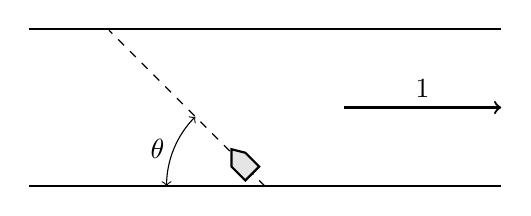
\begin{tikzpicture}
        %% River
        \draw[thick] (-3,1) -- (3,1);
        \draw[thick] (-3,-1) -- (3,-1);
        \draw[thick,->] (1,0) -- ++(0:2cm) node[anchor=south,pos=0.5] {\SI{1}{\meter\per\second}};
        %% Direction
        \draw[dashed] (0,-1) -- ++(135:2.8);
        \draw[<->] (-1.25,-1) arc (180:135:1.25) node[pos=0.5,anchor=east] {$\theta$};
        \node[fill=white!90!black,rectangle,minimum size=0.2cm,rotate=45,anchor=center] (M) at (-0.25,-0.75) {};
        %\draw (M.north west) -- ++(90:0.35) -- (M.north east);
        \path[draw,thick,fill=white!90!black] (M.north west) -- ++(90:0.22) -- (M.north east) -- (M.south east) -- (M.south west) -- cycle;
        %% NOTE: add riples in river
    \end{tikzpicture}
    \end{center}
    At what angle $\theta$ should he point the bow (front) of his boat?
    \begin{multicols}{3}
    \begin{choices}
        \wrongchoice{\ang{30}}
        \wrongchoice{\ang{45}}
        \wrongchoice{\ang{60}}
        \wrongchoice{\ang{63}}
      \correctchoice{\ang{90}}
    \end{choices}
    \end{multicols}
\end{question}
}

%% NOTE: Not mulitple choice
%\element{halliday-mc}{
%\begin{question}{halliday-ch04-q45}
%    A girl wishes to swim across a river to a point directly opposite as shown. 
%    She can swim at \SI{2}{\meter\per\second} in still water and the river is flowing at \SI{1}{\meter\per\second}. 
%    \begin{center}
%    \begin{tikzpicture}
%        %% NOTE: picture
%    \end{tikzpicture}
%    \end{center}
%    At what angle $\theta$ with respect to the line joining the starting and finishing points should she swim?
%    \begin{multicols}{2}
%    \begin{choices}
%      \correctchoice{}
%    \end{choices}
%    \end{multicols}
%\end{question}
%}

\endinput


